\documentclass[sigconf]{acmart}
\sloppy
\usepackage{graphicx}
\usepackage{color}
\settopmatter{printacmref=false} % Removes citation information below abstract
\renewcommand\footnotetextcopyrightpermission[1]{} % removes footnote with conference information in first column
\pagestyle{plain} % removes running headers
\makeatletter
\renewcommand\@formatdoi[1]{\ignorespaces}
\makeatother
\settopmatter{printacmref=false}

\usepackage{booktabs} % For formal tables
\setcopyright{none}

\newcommand{\MITAffiliation}{
\affiliation{%
  \institution{Massachussets Institute of Technology}
  \streetaddress{32 Vassar Street}
  \city{Cambridge}
  \state{Massachussets}
  \country{USA}
  \postcode{02139}
}}
 
 \newcommand{\EPFLAffiliation}{
\affiliation{%
  \institution{Swiss Federal Institute of Technology in Lausanne (EPFL)}
  \streetaddress{Route Cantonale}
  \city{Lausanne}
  \country{Switzerland}
  \postcode{02139}
}}

\newcommand{\srm}[1]{\textcolor{red}{{\bf Sam:} #1}}
\newcommand{\ra}[1]{\textcolor{blue}{{\bf ra:} #1}}
\newcommand{\gl}[1]{\textcolor{violet}{{\bf Gl:} #1}}
\begin{document}
\title{ShrinkNets}

\author{Guillaume Leclerc}
\authornote{Visiting Student}
\MITAffiliation
\email{leclerc@mit.edu}

\author{Raul Castro Fernandez}
\MITAffiliation
\email{raulcf@csail.mit.edu}

\author{Samuel Madden}
\MITAffiliation
\email{madden@csail.mit.edu}


% The default list of authors is too long for headers.
\renewcommand{\shortauthors}{G. Leclerc et al.}


%\begin{abstract}
%  Write the abstract at the end !
%\end{abstract}

\maketitle

\section{Introduction}

When designing Neural Networks, finding the appropriate size (width and depth)
is key. In particular, these hyper parameters have a strong correlation with
over/underfitting \srm{give reference} \gl{I did some litterature review and
  actually this statement is quite controversial, should we rephrase ?}. We
have no reliable way to find them but decades of experimentation led to some
heuristics ~\cite{Bengio2012a} that try to prune that immense space of possible
network sizes and suggest range of values to explore. To select the best
candidates , researchers have used strategies such as random search \gl{Should
  we also move the references here if we remove the pargraph from the related
  work ?}, meta-gradient descent ~\cite{Pedregosa2016} and Parzen Estimators
~\cite{Bergstra2011a} to reduce find good parameters without exhaustively
exploring the entire hyper-parameter space. Although these strategies help with
finding a good set of hyper-parameters, they still require a compute-intensive
search of the space.

%However, we are still bound to use costly and sometimes complex methods to
%find reasonable values for these hyper-parameters.

In this paper we present a method to automatically find an appropriate network
size from a single parameter, drastically reducing the hyper-parameter
dimensionality. The key idea is to \emph{learn} the right network size at the
same time that the network is learning the main task. For example, for an image
classification task, with our approach we can provide the training data to a
network---without sizing it a priori---and expect to end up with a network that
has learnt the task without overfitting \gl{too strong, we do not really have
  any guarantee on the generalization, how about changing it to: to end up with
  a network that learnt a tradeoff between size and accuracy}. This approach
has two main benefits. First, we do no longer need to choose a network size
before training.  Second, the final network size will be appropriate for the
task at hand, and not larger \gl{Should we talk about the fact that it automatically gets rid of dead neurons ?}. This is important because oversized networks have
a lower inference throughput and higher  memory footprint.

Our approach has two main challenges. First, on how to dynamically size the
network during training. Second, on how to find a loss function that optimizes
for the additional task of sizing, without deteriorating the learning
performance of the main task. We describe next ShrinkNets, which cope with both
challenges:

% \subsection{Main Contributions}
% 
% The main contribution of this article are:
% \begin{itemize}
%   \item The Filter layer, a neural network layer which puropose is to allow feature selection
%   \item To the best of our knowledge, the first attempts to dynamically change the number of channels in deep convolutional neural networks
%   \item A deep learning library built on top of PyTorch that allow partictionners to train shrinking networks (Feed-Forward and Convolutional)
% \end{itemize}
% 

\section{ShrinkNets}

Our approach consists of starting the training process for the task of interest
with an explicitly oversized network. Then, as training progresses, we learn
which neurons are not contributing to learning the main task and remove them
dynamically, thus shrinking the network size. This method requires two building
blocks. First, a way of identifying neurons that are not contributing to the
learning process, and second a way of balancing the network size and the
generalization capability for the main task. We introduce a new layer, called
\textsf{Filter}, which takes care of \emph{deactivating} neurons. We also modify
existing loss functions to incorporate a new term that takes care of balancing
network sizing and generalization capability appropriately. We explain them
next:

%\subsection{Motivation}
%
%\srm{This makes what we have done sound like an incremental change over prior
%work.  Instead, move this description to prior work and say why its not a good
%approach there, then describe what we do as a new method.  }
%
%The method described in [ref] grows and shrinks the network over time. Though
%this seems to be an attractive property to have, during our experiments and
%according to their results, models are very slow to train and sometimes
%converge to suboptimal solutions. Their method also requires a new optimizer
%\textit{AdaRad}.  Our goal was to provide a solution that can easily be
%integrated in existing machine learning systems and provide similar convergence
%speed and accuracy. Therefore, designing a new layer that only allow shrinking
%seemed to be best approach.
%

%\subsection{Definition}

\textbf{Filter Layers: } They have weights in the range $[0,+\infty]$ and are placed after
linear and convolutional layers of traditional deep networks \gl{This is how I
  used it but with the new implementation we can be more creative and put them
  anywhere, should we say "usually placed" insdead ?}. The \textit{Filter
  Layer} takes an input of size $\left(B \times C \times D_1 \times \dots
  \times D_n\right)$, where $B$ is the batch size, $C$ the number of features
(or channels), and $D$ any additional dimension. This structure makes it
compatible with fully connected layers with $n=0$ or convolutional layers with
$n=2$. Their crucial property is a parameter $\theta \in \mathbb{R}^C$, defined
as follows:

\begin{equation} Filter(I;\theta) = I \circ \max(0, \theta) \end{equation}

Where $\circ$ is the Hadamard product (pointwise multiplication \gl{Should we
  keep only one of them to be more concise ?}), and $\theta$ is expanded in all
dimensions except the second one to match the input size. It is easy to see
that if for any $k$, if $\theta_k \leq 0$, the $k^{\text{th}}$ feature/channel
will forever be $0$. When this happens, we say the Filter layer disables the
neuron. These disabled neurons/channels can be removed from the network without
changing its output (we describe how we perform this removal below). We explain
next how the weights of the Filter Layer are adjusted during training.

%We can use this property to devise a training procedure.

%To train networks we need start with a substantially oversized network, then we
%insert \textit{Filter Layers}  (usually after every linear or convolutional
%layer except the last one) and we sample their weight from the
%$\text{Uniform}(0, 1)$ distribution. 

%The \textit{Filter Layer} takes an input of size $\left(B \times C \times D_1
%\times \dots \times D_n\right)$ so it is compatible with fully connected layers
%with $n=0$ or convolutional layers with $n=2$. This layer has a parameter
%$\theta \in \mathbb{R}^C$ and is defined the following way. \srm{Need to define
%B, C, D}.  
%
%\begin{equation} 
%Filter(I;\theta) = I \circ \max(0, \theta)
%\end{equation}
%
%Where $\circ$ is the Hadamard product (pointwise multiplication), and $\theta$
%is expanded in all dimensions except the second one to match the input size. It
%is easy to see that if for any $k$, if $\theta_k \leq 0$, the $k^{\text{th}}$
%feature/channel will forever be $0$. We can use this property to devise a
%training procedure.  
%
%\srm{Give an English description of what this formalism
%achieves -- what does the filter layer do, why is it significant.}

%\subsection{The training procedure}
\textbf{Training Procedure: } Once Filter layers are placed in a deep network, 
%To train networks we need start with a substantially oversized network, then we
%insert \textit{Filter Layers}  (usually after every linear or convolutional
%layer except the last one) and we sample their weight from the
%$\text{Uniform}(0, 1)$ distribution. 
we could train it directly and it
would be equivalent to a normal neural network. However, our goal is to find the
smallest network with reasonable performance. We achieve that by introducing
sparsity in the parameters of the \textit{Filter Layers}. Indeed, having a negative component in the $\theta$ parameter of the filter layer permamently disable its associated feature \gl{Maybe redundant ? we talked about that in the previous paragraph}
. To obtain this sparsity, we simply redefine the loss function:

\begin{equation}
  L'(x,y;\theta) = L(x, y) + \lambda|\theta|
\end{equation}

This choice come from the Lasso loss ~\cite{Tibshirani1996} and we use it for the same reason:
it introduces sparsity. The bigger the $\lambda$ the more entries in $\theta$
are set to zer0, and since zero entries in $\theta$ correspond to dead neurons,
lambda effectively control the number of neurons/channels in the entire
network.
Next, we explain how to implement ShrinkNets efficiently.

\textbf{Software architecture\footnote{The code is available as Python/PyTorch
    library on \url{http://github.com/mitdbg/fastdeepnets} \gl{Should we rename
      the repository ?}}: }\textit{Filter Vectors} can easily be implemented in
a few lines of code in many existing deep learning frameworks. However, in
ShrinkNets, we assume that we start with obviously oversized networks. If
disabled neurons are not quickly removed, the overhead might cause the training
process to be significantly slower than classic neural networks. This is why we
want to support what we call garbage collection: removing the weights in the
layers that are responsible (or using) features that are disabled.  \par To be
able to catpure this relationship between layers, we agumented \textit{Pytorch}
~\cite{paszke2017automatic} (the framework we used as the
foundation of our implementation) with a graph structure very similar to the
one available in Keras ~\cite{chollet2015keras}.  In this graph, edges are
effectively event hubs responsible for propagating \textit{feature removal}
events to its endpoints. ShrinkNet layers are designed to emit and react to
these events but also propagate the event further if has an impact at the other
endpoint of the layer (input or output) \gl{What I mean here is: if the event
  comes from the output, it might be propagated to the inputs, and the other
  way around}.  \par This event-based implementation coordinated by edges makes
it very easy to integrate new layers in the library.  We even provide automatic
wrapping for layers from \textit{PyTorch} if they have no internal state. For
more complex ones, we provide utilitaries that
makes the implementation very concise.

\section{Evaluation}
\subsection{Convergence}

To demonstrate that the approach is viable, we will first show that Shrinking
Networks converge properly. For this experiment we trained a one hidden layer
neural network with one filter layer to control the number of hidden units. We
initialized the models with $10000$ neurons and trained them on \texttt{MNIST}
~\cite{Lecun1998} using different regularization factors ($\lambda$). We
summarized the results in \autoref{convergence_plot}. We can see on this plot
is that for a given $\lambda$ the number of hidden units seems to always
converge to some value. It has two implications: it seems that $\lambda$ is, as
we would think, a proxy of the network size (bigger $\lambda$ imply smaller
networks). Secondly, it indicates that the spikes we see in the regular spikes
we see in the loss that occur when neurons are disabled will eventually
disapear because the number of neurons reach a plateau. \gl{I feel we should
  give a conclusion for this paragraph but I am not sure what to say}
\begin{figure}
\begin{center}
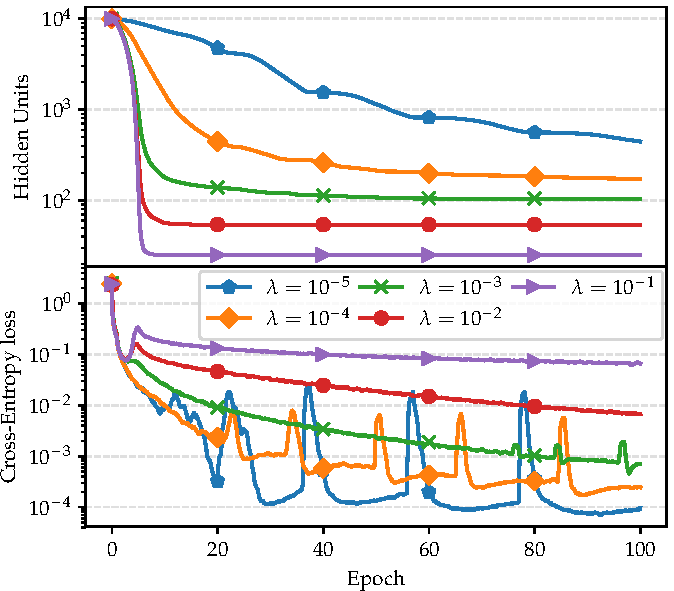
\includegraphics[width=0.5\textwidth]{convergence}
\caption{Evolution of the number of hidden units and loss over time on the \texttt{MNIST} dataset for different $\lambda$ values \label{convergence_plot}}
\end{center}
\end{figure}


\subsection{Relevance in the context of hyper-parameter optimization}

One of our main goal is to help finding neural network architectures that
perform reasonably well faster than existing techniques. For simplicity, we
will try to see how ShrinkNets perform when doing random search over a sub set
of the hyper-parameter space (we will fix everything except the size-related
parameters). However, we believe that the results generalize to more complex
methods, most of them might actually benefit a lot from the reduction of the
dimensionality of the hyper-parameter space.

\par To isolate the effect of ShrinkNets we will consider two very simple
architectures: multi-layer perceptrons (with three hidden layers) and the
\textit{LeNet-5} model ~\cite{Lecun1998}. For this experiment we assume we have no prior
information about the size except an upper bound of $50$ channels per
convolutional layer and $5000$ neuron for fully connected layers.  We try to
find the appropriate size of the network using classical neural networks and
ShrinkNets. To make sure that we are as fair as possible and since one might
argue that ShrinkNets is also regularizing the network in addition to finding
the size, we will also considered regularized classic networks using the most
commonly used technique: the $L_2$ penalty ~\cite{Ng2004}.
\par The experiment consist in sampling parameters randomly for each class of
network, train them for the same amount of epochs (100 for MLPs and 200 for CNNs). Pick the epoch that performed the best on the validation set and evaluate it
on the testing set. We repeat the process for 50 models. This evaluation was done
on \texttt{MNIST} ~\cite{Lecun1998}, \texttt{FashionMNIST} ~\cite{Xiao2017} and \texttt{CIFAR10} ~\cite{Krizhevsky2009}. The distribution of the testing accuracy we obtained is summarized on \autoref{hyper_opt_res}.

We can see that the distributions for ShrinkNets are consistently better than the
others for all datasets and both architectures. It shows that by training fewer
networks, we are likely to obtain on-par or even better models which effectively
reduces the cost of hyper-parameter optimization. In some cases the best ShrinkNets
models even outperforms the best model of the other techniques.

\begin{figure}
\begin{center}
  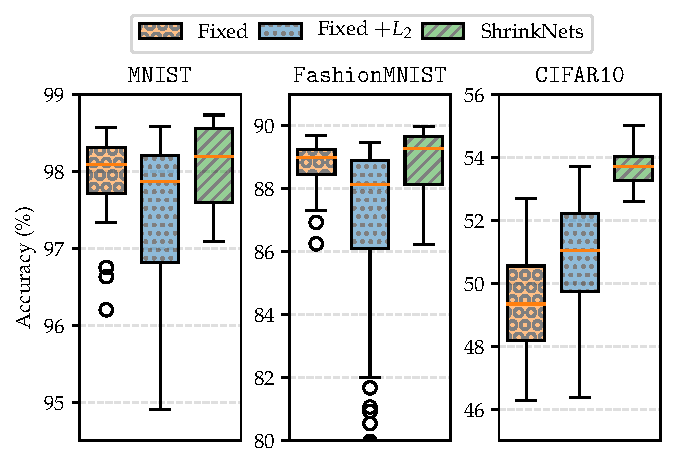
\includegraphics[width=0.5\textwidth]{hyper_opt}
\caption{Distributions of the testing accuracy for different training methods, datasets and architectures using random search\label{hyper_opt_res}}
\end{center}
\end{figure}

\section{Related Work}

\par There are many methods in the litterature that try to simplify the neural
network structure. Most of them focuses on removing connections (eg: ~\cite{Cun},
~\cite{Han2015}).  However, most hardware (GPU's, TPUS ~\cite{Jouppi2017}, TensorCores) do not really
leverage sparsity in the connections efficiently (as explained in ~\cite{Han2016}). On the other side, ShrinkNets
and some others ~\cite{Scardapane2017} and ~\cite{Philipp} try to remove entire neuron instead of
connections. This is very usefull because it reduces the size of the matrices,
producing speed-up on every device. ShrinkNets improves on
~\cite{Scardapane2017} because it removes neurons during training, speeding up
the rest of the process and beats ~\cite{Philipp} on convergence speed and because it
does not need to change the optimizer. To the best of our knowledge this is
also the first contribution that tries to learn the number of channels of a
convolutional neural network.

\section{Conclusion}

In this paper we presented a novel technique to guess a resonable network size
based on single parameter $\lambda$ that control the tradeof between loss and
the size. We demonstrated that it works both on fully connected networks and
convolutional neural networks.  Even though the firsts results seem promising,
there are many ways we could improve. In the current implementation we only
"learn" the number of features (neurons or channels). We could try to augment
it with dynamic number of layers as seen in ~\cite{meier} to be able to
determine the entire architecture. \par We saw on Figure \ref{convergence_plot}
that the loss temporarily suffers from the removal of neurons. It is likely
that the loss would be more stable if the number of neurons converged faster or
neurons disappeared slower. For this reason we plan to explore proximal
gradient methods to optimize the filter vectors and/or randomize neuron
removals. \par During our evaluation we picked small datasets mainly to be able
to train many models and have statistically significant distributions. With
more computation resources and time, we could see if it generalizes to bigger
datasets and other architectures like \texttt{ResNet} ~\cite{He2016} (small
modifications to the existing code base are required to support them)

\bibliographystyle{ACM-Reference-Format}
\bibliography{bib,custom}

\end{document}
